-\section{Struttura centrale}

Durante lo sviluppo del prodotto, in fase di progettazione, che ha lo scopo di identificare le caratteristiche funzionali e comportamentali dell’applicazione, vengono evidenziate le parti principali del programma con le relative funzioni assolte.\\
\\
Le prime scelte della fase successiva, l’implementazione, riguardano l’architettura e le tecnologie del sistema. La loro relazione specifica il comportamento dei componenti e determina le modalità con cui si interfacciano tra loro.\\
\\
L’abilità di trovare le migliori soluzioni che più si adattano alla risoluzione delle esigenze rispettando i requisiti espressi in fase di progettazione comporta fin da subito uno sviluppo corretto ed efficiente.  \\
\\

\begin{figure}[h!]
    \centering
    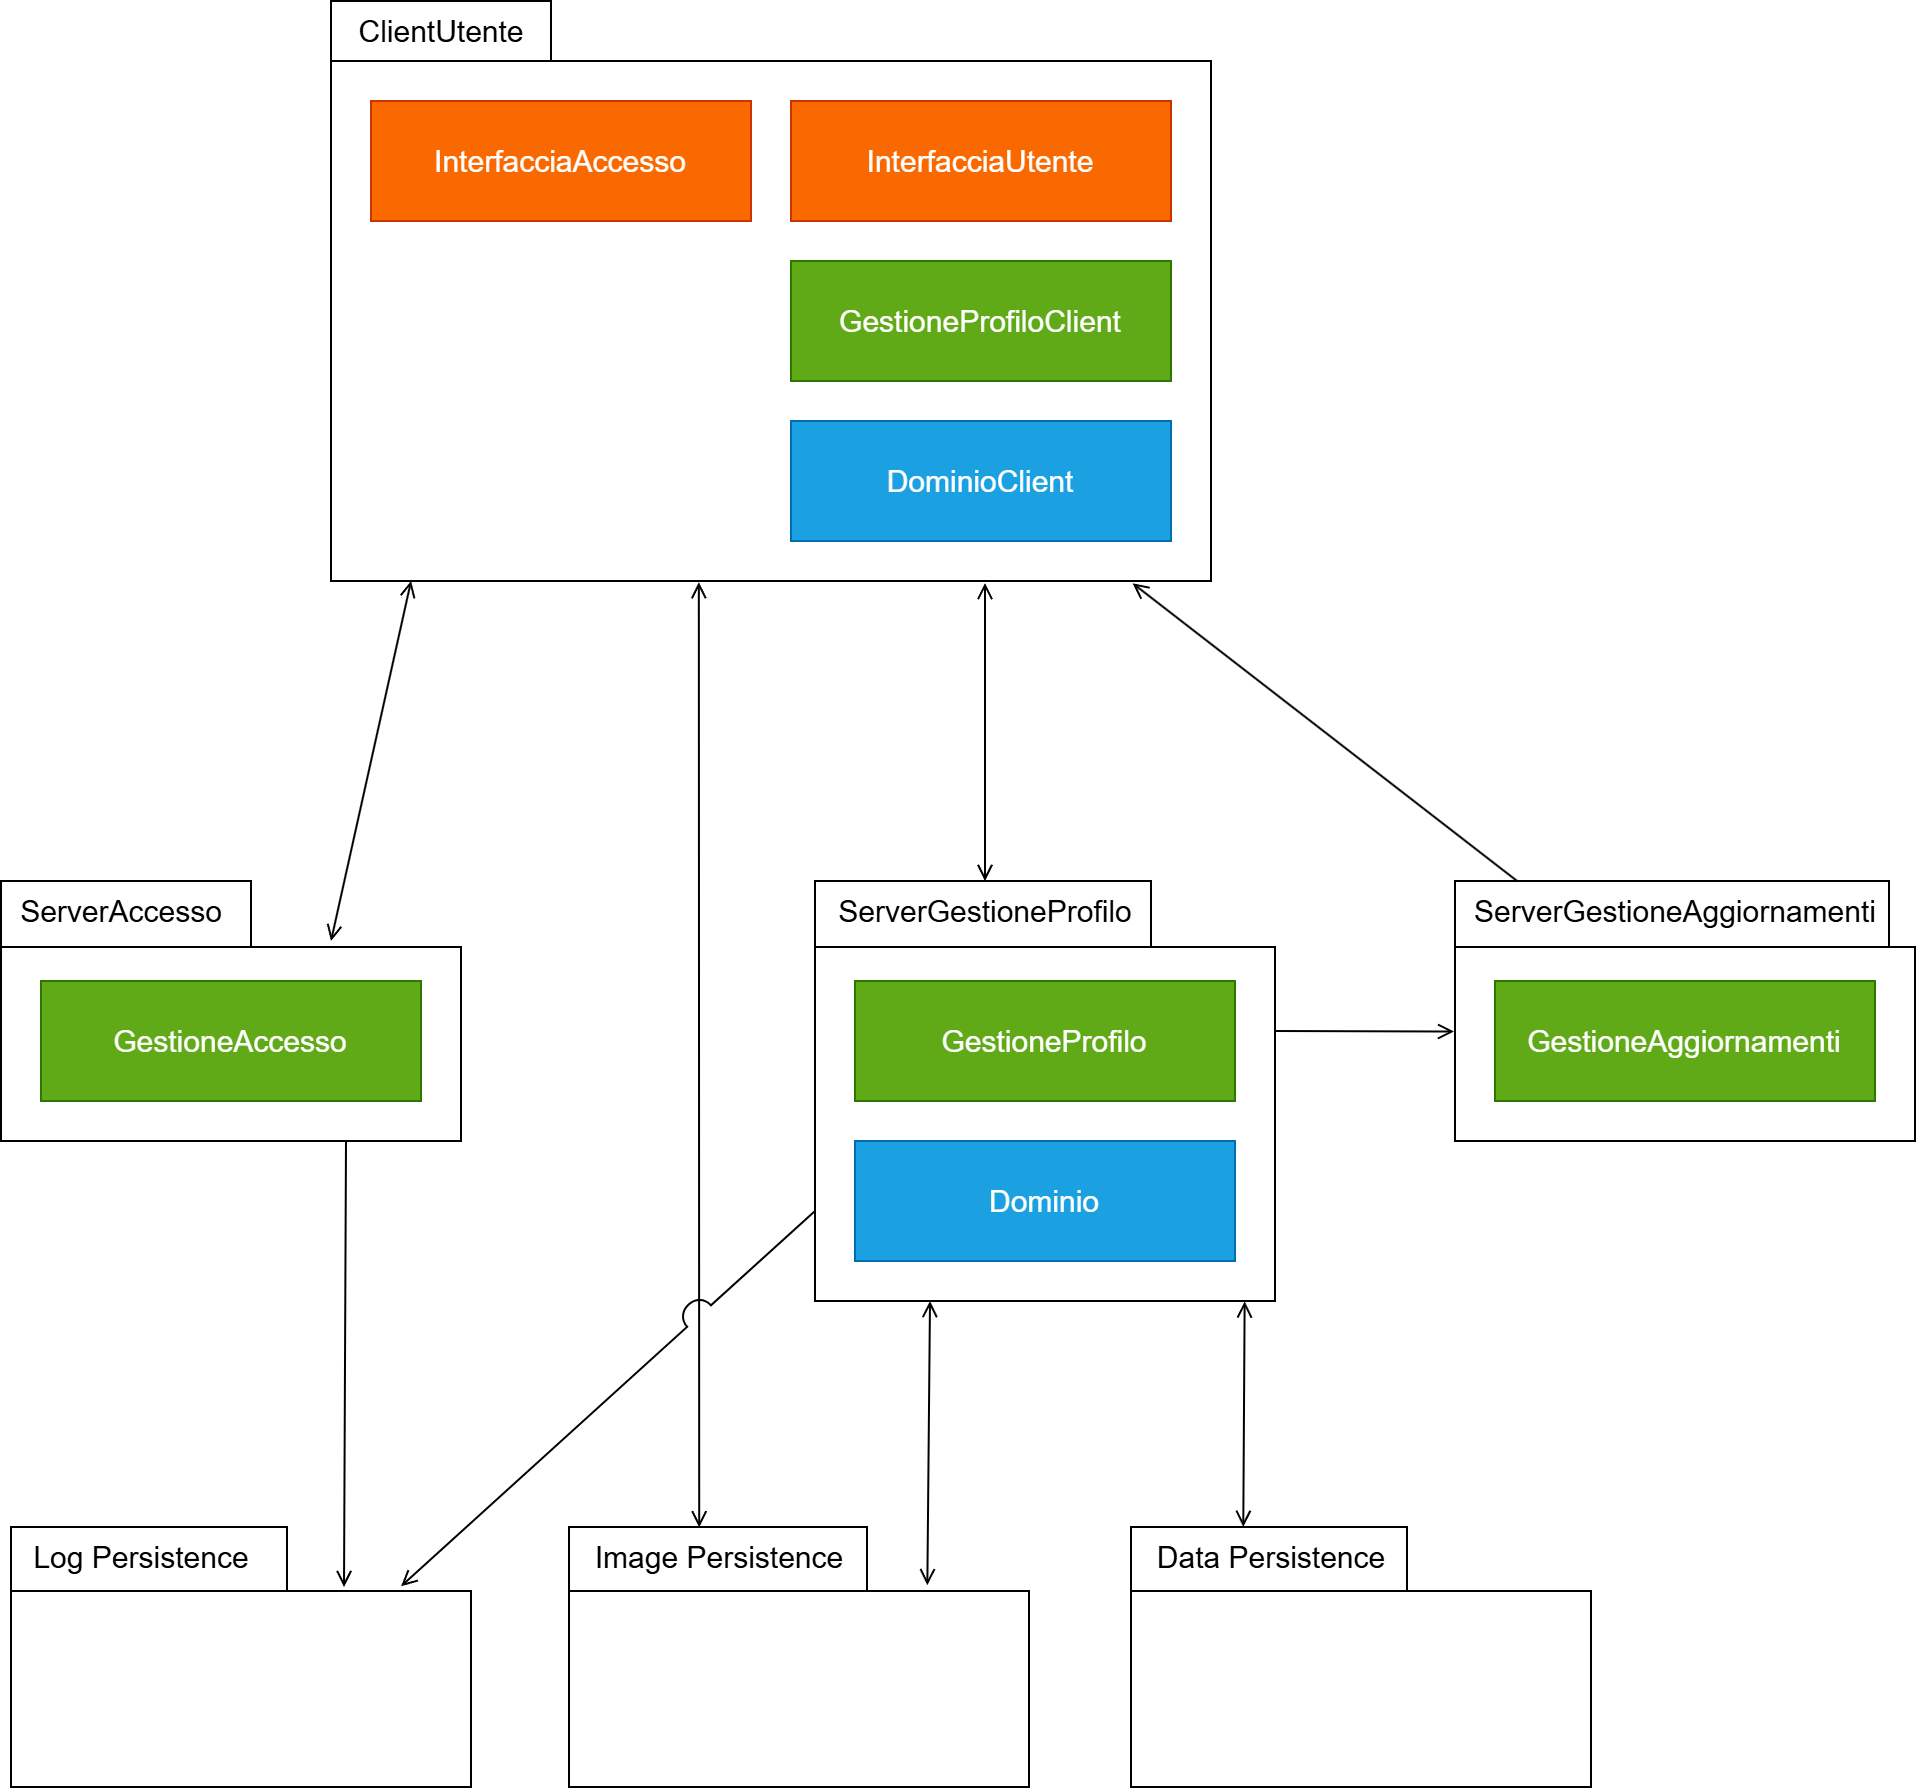
\includegraphics[width=\textwidth]{ProgettoDiagrammaPackage.png}
    \caption{Struttura e responsabilità delle parti del progetto}
\end{figure}
Sebbene per alcune parti le decisioni possano risultare semplici o intercambiabili, altre possono dover richiedere ulteriori analisi. Risulta conveniente sviluppare prima i componenti di cui sono ben definiti i requisiti ed è presente una soluzione chiara che risponde alle esigenze specifiche. L’identificazione, anche parziale, di una struttura iniziale determina ulteriori requisiti di integrazione che facilitano l’individuazione delle restanti soluzioni necessarie.

\clearpage
\subsection{Sviluppo del Client}

L’utilizzo delle applicazioni per la gestione degli eventi può essere suddiviso in due fasi distinte, ciascuna con specifiche esigenze funzionali. 
La prima fase riguarda infatti la pianificazione a lungo termine e l’organizzazione degli impegni. In questo tempo l’utente decide come distribuire il proprio tempo, pianificando attività e appuntamenti, e strutturando il proprio calendario nel modo più efficiente per le proprie necessità. 
La seconda fase riguarda invece la gestione degli eventi non ancora certi e definiti; ciò include l’invito a un evento, l’eventuale conferma da parte dell’utente, l’identificazione degli impegni a breve termine e l’aggiornamento del loro stato (ad esempio, se l’evento sia ancora confermato, quante persone vi partecipano, se qualcuno ha annullato o se l'evento è già concluso) con la gestione degli eventuali contenuti multimediali successivi all’evento. Queste due fasi implicano un approccio diverso da parte dell’utente, comportando di conseguenza esigenze differenti a cui l’applicazione deve rispondere adeguatamente. 
Per rispondere a tali necessità, è fondamentale che l'applicazione offra un'interfaccia utente versatile, fruibile sia da desktop che da dispositivi mobili. La versione desktop consente una pianificazione a lungo termine, offrendo una visione d'insieme chiara e completa di tutti gli impegni, tale da facilitare la gestione del tempo. D'altra parte, la versione mobile deve permettere una gestione rapida e dinamica degli eventi quotidiani, garantendo che l'utente possa rimanere sempre connesso e aggiornato sugli sviluppi in tempo reale.
Inoltre, considerando che l'applicazione è destinata a un utilizzo diffuso e a un'utenza potenzialmente elevata, è necessario garantire tempi di risposta ridotti e una gestione efficiente delle richieste concorrenti. Ciò implica la progettazione di un sistema in grado di scalare facilmente, per supportare un ampio numero di utenti simultanei senza compromettere le prestazioni.

Al fine di ottenere tutte le prestazioni precedentemente elencate, la scelta è ricaduta sull’adozione del framework di sviluppo Flutter. Diversi fattori motivano tale decisione. 
In primo luogo, l'architettura di Flutter si basa su un motore grafico indipendente dalla piattaforma di esecuzione, il che consente di ottenere elevate prestazioni e garantire un'esperienza utente uniforme su dispositivi diversi. 
In secondo luogo, Flutter adotta un approccio dichiarativo nella progettazione dell'interfaccia grafica, che facilita lo sviluppo di componenti reattivi e scalabili attraverso un codice conciso, facilmente manutenibile.
Un ulteriore vantaggio di Flutter è rappresentato dalla crescente adozione nel settore, dalla solidità della community di sviluppo e dal supporto offerto da Google, che ne assicurano la stabilità, l'efficienza, la sicurezza e la disponibilità di componenti personalizzabili per l'intero ciclo di vita del prodotto. 
Infine, Flutter consente uno sviluppo rapido e interattivo grazie alla sua sintassi intuitiva e al meccanismo di hot reload, che riduce significativamente i tempi di compilazione e facilita il testing in tempo reale.

Tra le altre tecnologie valutate per lo sviluppo dell'interfaccia grafica, vi erano React Native e Xamarin. Tuttavia, entrambe presentano alcune limitazioni: le applicazioni finali sviluppate con React Native tendono ad avere dimensioni più elevate e le prestazioni risultano inferiori, in particolare nella gestione della memoria. Xamarin, pur essendo una valida opzione, presenta una curva di apprendimento più ripida e una comunità di sviluppatori più ridotta rispetto a Flutter, con una conseguente minore disponibilità di componenti e librerie.

Per quanto Flutter consenta di uniformare l'esperienza utente su dispositivi diversi e semplifichi la compilazione per le varie piattaforme, alcune configurazioni rimangono comunque dipendenti dalla tecnologia su cui l'applicazione viene eseguita. Di conseguenza, ciascun eseguibile richiede una manutenzione aggiuntiva, inclusi gli aggiornamenti delle dipendenze specifiche, sia a livello di deployment che di gestione delle versioni.

In una fase iniziale dello sviluppo, nell'ottica di coprire il più ampio mercato possibile con il minor numero di piattaforme, si è deciso di sviluppare una versione fruibile via web e una per dispositivi Android.

 Nell'ambito delle tecnologie Azure, per la  distribuzione del codice web è stato scelto Azure Static Web App, un servizio che permette di ospitare un sito web che non presenta caratteristiche dinamiche, ovvero nel quale la pagina restituita non varia in base all’utente che la richiede. L’applicazione in questione, per scelte progettuali, richiede i dati specifici dell’utente (se non li ha già in una cache locale) solo al server, rendendo l’interfaccia grafica completamente indipendente dall’utente che ne usufruisce.
La robustezza del servizio garantita dalla firma Azure e il suo prezzo ridotto per un uso limitato del servizio sono state ritenute caratteristiche sufficienti per la sua selezione.

Infine, in attesa della pubblicazione dell’applicazione sull’App Store di Android, l’esecutivo è stato reso disponibile tramite Azure Storage Container, un servizio che permette il salvataggio di file di differenti tipologie, allegando un link per il recupero. 

Il codice distribuito sulla web app e l'applicativo salvato sul container verranno aggiornati automaticamente tramite GitHub Actions.
Nella fruizione tramite browser il codice si aggiorna ad ogni accesso, mentre l'applicativo necessita di venire re-installato. Per questa ragione, gli utenti che usano l'applicazione verranno notificati nel momento del caricamento di una nuova versione.

\clearpage
\subsection{Architettura del server principale}
	
L’applicazione necessita della capacità di rispondere a quantità elevate di richieste in breve termine. In altre parole, deve essere scalabile. 
Il servizio Azure che meglio risponde a questa esigenza è Azure Functions. Azure Functions è una risorsa che permette di suddividere il codice in nuclei indipendenti tra loro, creando un ambiente di esecuzione unico per ogni richiesta. Questa caratteristica, unita alla virtualizzazione dell’ambiente di esecuzione fornita dai servizi in cloud, rendono possibile una scalabilità potenzialmente infinita.

La responsabilità dell’indipendenza di ogni funzione e della sua proprietà di essere stateless(ovvero svincolata dal contesto in cui viene eseguita, senza conoscenze dello stato o della sessione), ricade sullo sviluppatore. Ogni funzione assolve un unico compito, seguendo il principio di singola responsabilità. Nel caso in cui una richiesta richieda l’esecuzione di più compiti, Azure Function mette a disposizione la tecnologia Azure Durable Functions. 

Integrata all’interno delle AF, Azure Durable Function permette la creazione di una funzione orchestrator che gestisce l’ordine, lo stato, il tempo di vita e le risposte delle varie funzioni da eseguire per soddisfare la richiesta.
Rimanendo nell’ottica di un ambiente indipendente e scalabile, consente di gestire situazioni in cui l’ordine dei compiti è importante, siano richiesti ulteriori tentativi in caso di fallimento o sia necessaria l’attesa del completamento dei compiti con un tempo di esecuzione elevato.
Per loro natura, le Azure Durable Functions presentano però un tempo di risposta più elevato, a causa della natura stateless e quindi dell’accoppiamento debole con le funzioni che sta eseguendo.  
Grazie a questa tecnologia verranno inizializzate solo le funzioni strettamente necessarie per l’esecuzione di un determinato compito, stanziando al minimo le risorse effettivamente necessarie.

Come linguaggio di programmazione per lo sviluppo delle funzioni è stato utilizzato C\#. L’integrazione con Entity Framework Core permette di mappare direttamente in oggetti i componenti del dominio, semplificando la logica delle relazioni e astraendo le comunicazioni con il database. Grazie all’utilizzo delle proprietà virtuali degli oggetti si rende inoltre possibile il lazy loading, per il quale le richieste al database avvengono solo quando strettamente necessarie. Infine, la consapevolezza che sia l’ambiente di sviluppo di C\#, ovvero il framework .Net, sia la piattaforma Azure sono mantenute dalla stessa azienda, ovvero Microsoft, garantisce il supporto, la stabilità e l’integrazione delle tecnologie.

La piattaforma di sviluppo Visual Studio Code fornisce inoltre la possibilità di collegarsi direttamente ai servizi in cloud tramite estensioni apposite, che rendono l’aggiornamento del codice estremamente semplice e lineare, oltre che immediato.

Azure Function in ambiente .Net permette lo sviluppo in due modalità differenti: in-process worker o isolated worker. Si definisce worker l’applicativo che si occupa di creare le risorse ed eseguire le funzioni in base alle richieste. Nella modalità in-process la funzione eseguirà all’interno dello stesso processo del worker che l’ha creata, riducendo il numero di risorse necessarie ma condividendo l’ambiente di esecuzione. Nel modello isolated ogni funzione viene creata usando un processo unico dedicato, aumentando l’isolamento e quindi riducendo le possibili dipendenze tra le funzioni. Inoltre, il supporto al modello isolated prevede un maggior numero di versioni del framework .Net, che per il modello in-process sono limitate alle sole versioni con supporto a lungo termine. Infine, il supporto per la creazione di un middleware che esegua tra la chiamata e l’esecuzione di una funzione è supportato solo per il modello isolated. 
Per queste ragioni, si è deciso di sviluppare le funzioni usando il modello isolated.

\clearpage
\subsection{Autenticazione}

	La facilità di autenticazione è essenziale per l’esperienza utente. La possibilità di entrare nell’applicazione tramite il proprio authentication provider di fiducia è sicuramente apprezzata, ma allo stesso modo è essenziale offrire la possibilità di creare un account dedicato alla singola applicazione. Il servizio di gestione degli accessi dovrà quindi soddisfare sia l’esigenza di creare account nuovi mantenuti e controllati dall’applicazione, che fornire la possibilità di interagire con i diversi authentication providers.

Azure mette a disposizione il servizio Microsoft Entra ID, all’interno di una famiglia di servizi per l’autenticazione e l’autorizzazione chiamata Microsoft Entra. Per quanto dovrebbe essere in grado rispondere alle funzionalità di cui sopra, la confusione della documentazione e la difficoltà incontrata nell’integrazione con il servizio hanno portato a cercare un’altra soluzione negli ambienti cloud.

La risposta è stata trovata in Firebase Authentication, che garantisce la possibilità di creare account così come di collegarsi ad altri authentication providers. Inoltre, presenta un’interfaccia chiara e offre servizi di integrazione di facile utilizzo sia tramite Flutter che tramite C\#. A livello di costi, il servizio è gratuito sotto i cinquantamila utenti attivi mensilmente.

Tra i requisiti del progetto è richiesto che un account identifichi un solo utente. In fase di creazione del profilo, tuttavia, l’account viene salvato sulla persistenza del server Firebase. 
Si rende necessario, nel momento del primo accesso, che il server, dopo aver controllato l’autenticità della richiesta, crei una copia dell’account, così come il nuovo oggetto utente e il primo profilo relativo.
\begin{figure}[h!]
    \centering
    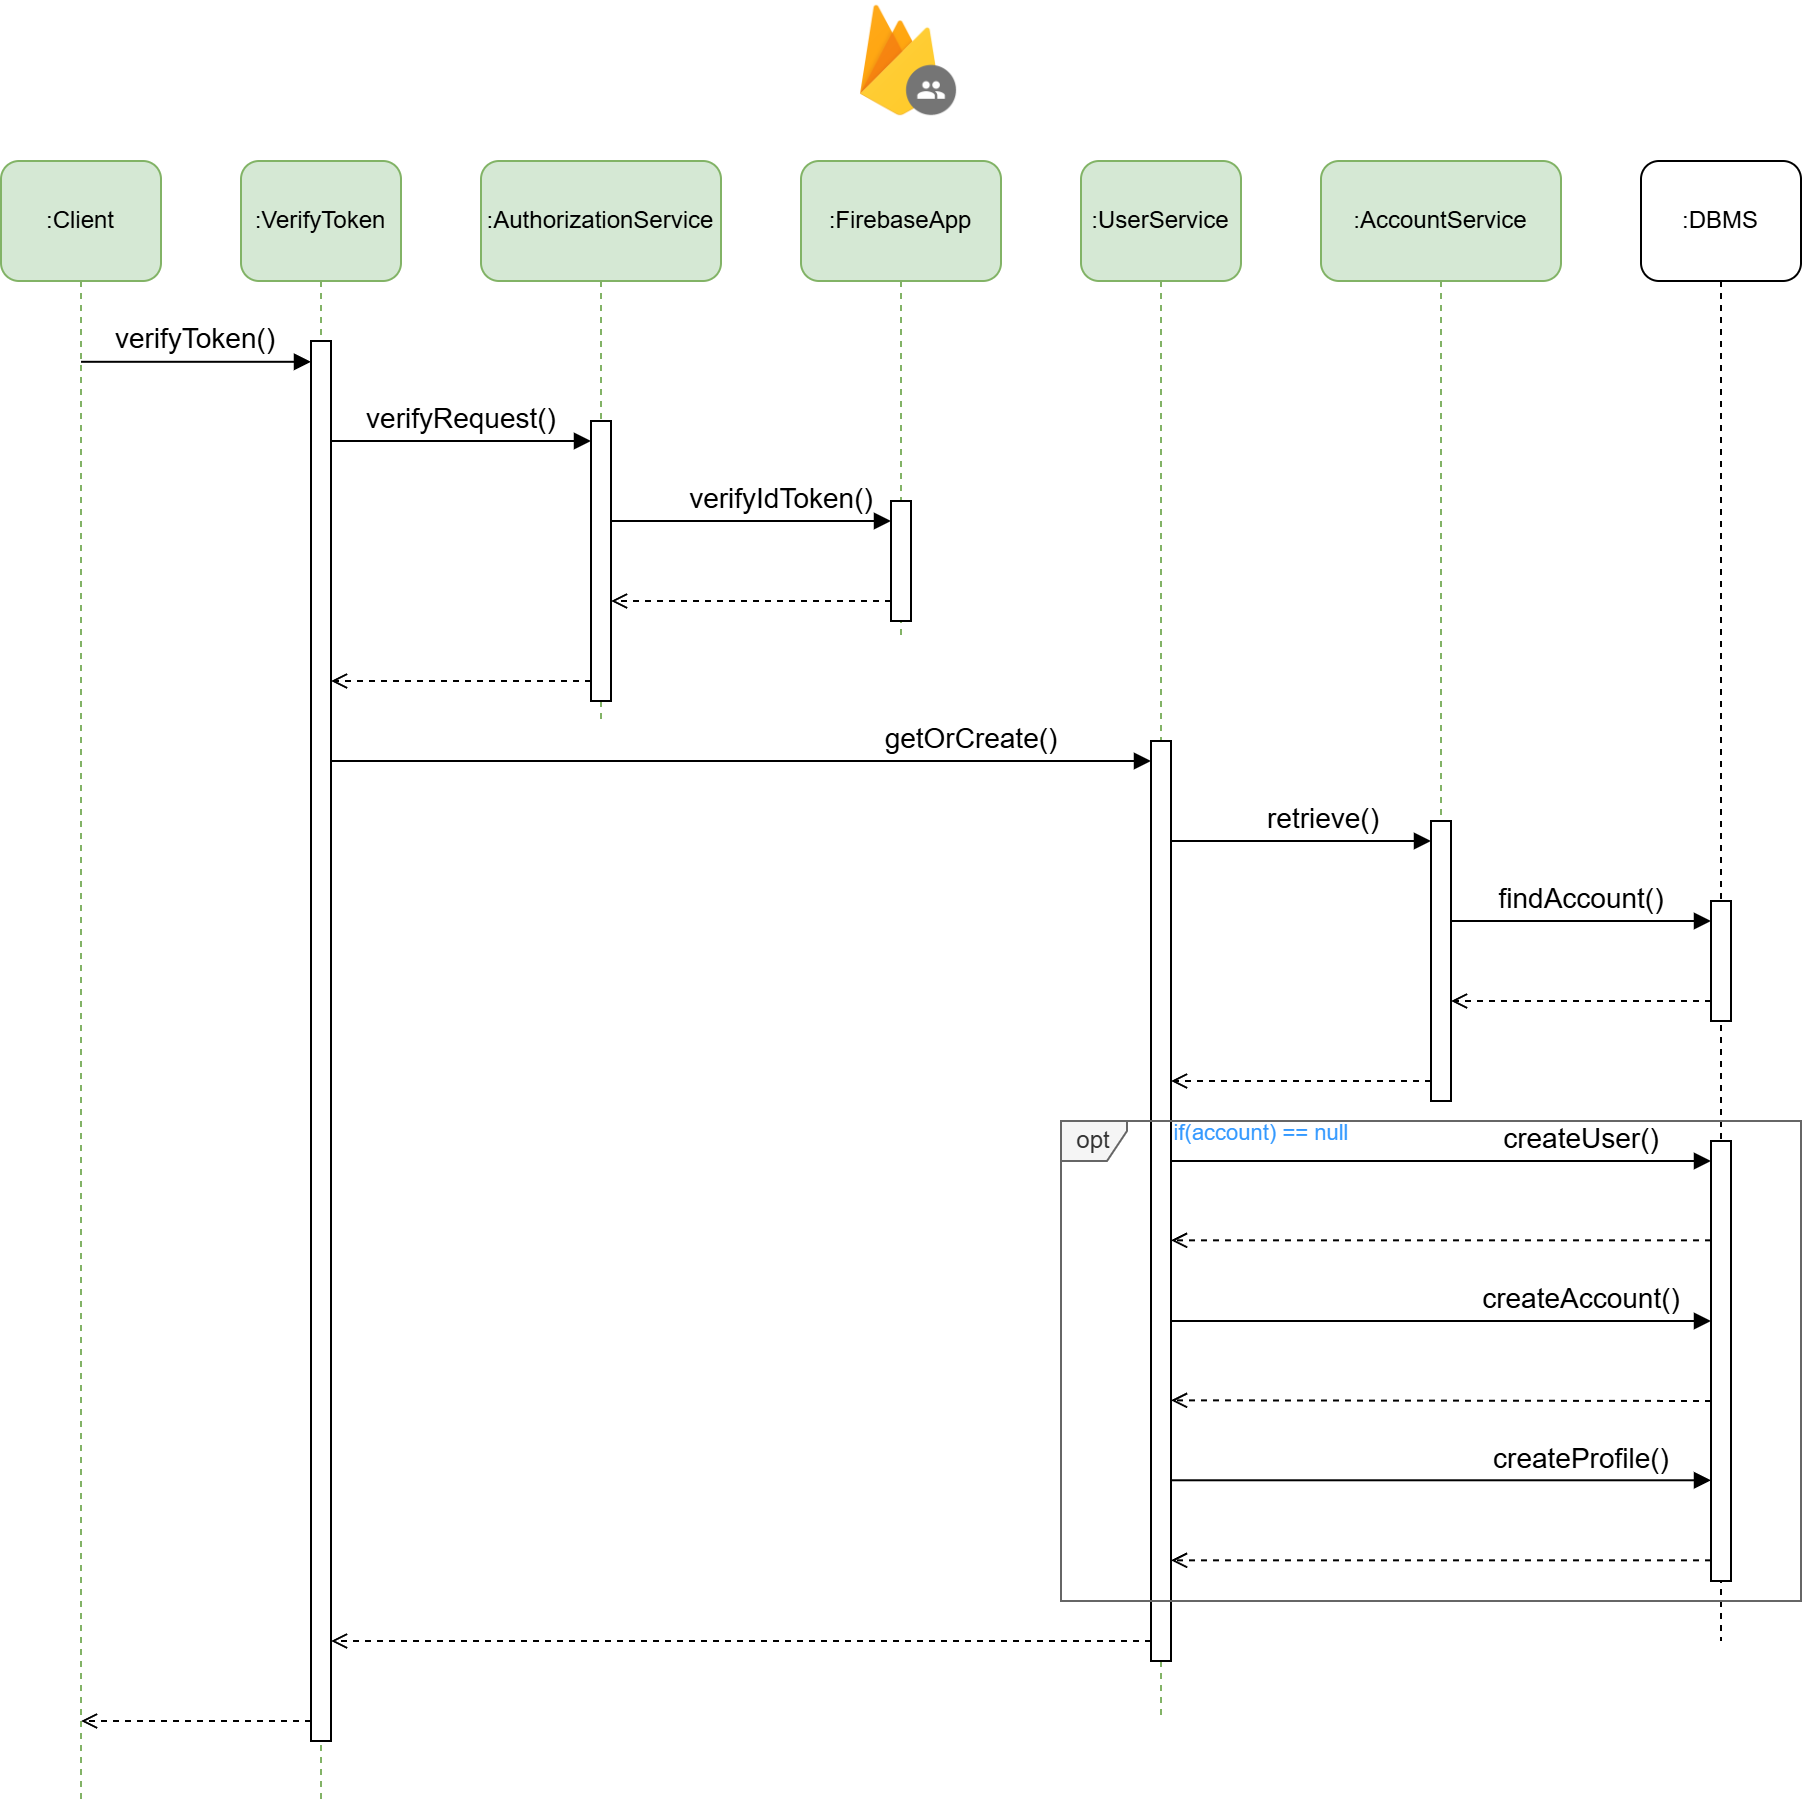
\includegraphics[width=\textwidth]{IIVerifyToken2.png}
    \caption{Diagramma di sequenza per la creazione di un account}
\end{figure}
Ad ogni richiesta in cui sia necessaria l’identificazione, il dispositivo utente aggiungerà alle richieste il token identificativo salvato a seguito dell’autenticazione iniziale. Il server controllerà che il token sia valido, per poi eventualmente proseguire l’esecuzione.


\clearpage
\subsection{Sicurezza}

Il collegamento tra i vari componenti all’interno dell’ambiente Azure richiede l’utilizzo di chiavi e stringhe di connessione. Il salvataggio di tutte le chiavi sensibili è stato affidato al servizio Azure Key Vault, un server che permette la centralizzazione dei dati, cifrando il contenuto e garantendo un controllo maggiore sul loro utilizzo. Quando necessario i servizi, in particolare le Azure Function, contatteranno il Key Vault per l’ottenimento delle chiavi necessarie, riducendo il rischio di un’intercettazione data magari da un errore durante lo sviluppo.

Le comunicazioni tra i vari componenti devono avvenire in sicurezza, garantendo autenticità e confidenzialità. Per questo motivo tutte le comunicazioni tra dispositivi client e i vari servizi utilizzano la tecnologia TLS, che permette di cifrare i messaggi grazie ad uno standard collaudato. In particolare, le comunicazioni tra i client e Azure Function, così come con Firebase Authentication e il server per la persistenza delle immagini, avvengono tramite protocollo HTTPS, mentre le comunicazioni con il server per gli aggiornamenti in tempo reale usano il protocollo WSS.

L’accesso al database è ristretto alle sole risorse Azure, garantendo l’isolamento dall’esterno, che comprometterebbe altrimenti l’affidabilità dei dati.

Infine, l’identificativo di ogni elemento del dominio è nascosto all’utente tramite la creazione di codici hash univoci che permettono comunque l’identificazione dell’oggetto senza rivelare ulteriori informazioni. In particolare, il caricamento delle immagini avviene grazie ad un link univoco dato dalla combinazione degli identificativi dell’evento e dell’immagine. Utilizzando i codici di hash diventa molto complicato il ritrovamento delle immagini senza essere a conoscenza dei codici, che non avendo natura incrementale ma distribuita rende indovinare un link valido.

\clearpage
\subsection{Monitoraggio}

Il monitoraggio del sistema è attuato in due modalità: tramite salvataggio dei log e controllo delle prestazioni del sistema.

Relativamente a Firebase Authentication vengono forniti con il servizio sia le interfacce
per il controllo delle prestazioni che la gestione dei log. Non è quindi richiesta alcuna ulteriore azione.

Per monitorare le Azure Functions sarà invece necessario collegare Azure Application Insights, servizio che provvede a controllare il funzionamento e la risposta del servizio. Una volta unito il servizio, infatti, Azure Application Insight permette la presentazione e l'analisi di numerose metriche, quali il tempo di risposta e il consumo di risorse. Consente inoltre di testare la risposta dell’applicativo simulando diversi scenari e riassumendo il loro comportamento.

La creazione dei log è invece delegata al programmatore, in quanto è necessario integrarli nel codice. Nel momento della creazione, ogni funzione riceve, tramite dependency injection, un servizio Logger che permette la creazione e il salvataggio dei log. Tali log saranno poi consultabili e analizzabili tramite l’interfaccia fornita da Azure Application Insight.

\clearpage